\documentclass{article}
\usepackage{graphicx} % Required for inserting images
\usepackage[rightcaption]{sidecap}
\usepackage[style=alphabetic]{biblatex}

\graphicspath{ {./images/} }
\addbibresource{sample.bib}

\title{Assignment 4 Report}
\author{Ole Rößler (7211)}
\date{December 2024}

\begin{document}

\maketitle
\tableofcontents

\newpage
\section{Design Exercise: Flight Booking System}

\subsection{Requirements}
This section talks about the functional and non-functional requirements of the flight booking system wanted by the ACME Organization. 
The main points given were about the given points considering (this will be a short overview about the task).

Short Description what the differences between function and non-function requirements are and I chose them (from the given context and my personal thought).

\subsubsection{Functional Requirements}
\begin{enumerate}

\item \textbf{Fetching Data:}
Periodically receive flight data updates from partner airlines (every hour).
\item \textbf{View Flights:}
The customer is able to see specific flight details. 
Therefore the customer enters a specific flight number/ flight ID and gets updates about the specified flight.
\item \textbf{Booking:}
The customer is able to book a flight on a desired flight as well as make a seat reservation on the airplane (Most airlines offer different price-tiers for seats). 
\end{enumerate}

\subsubsection{Non-Functional Requirements}
\begin{enumerate}
\item \textbf{Price Consistency:}
The system has to maintain consistency in pricing, therefore short term increases in flight-prices have to be avoided .
\item \textbf{Performance:}
Low latency for user interactions (response within seconds).
\item \textbf{Scalability:}
The system has to handle hundreds of thousands of concurrent users as well as hundreds of flights send in their data on the hour.
\item \textbf{Fault tolerance:}
The system has to be reliable.
\end{enumerate}

\subsection{System Architecture}
\begin{figure}
    \centering
    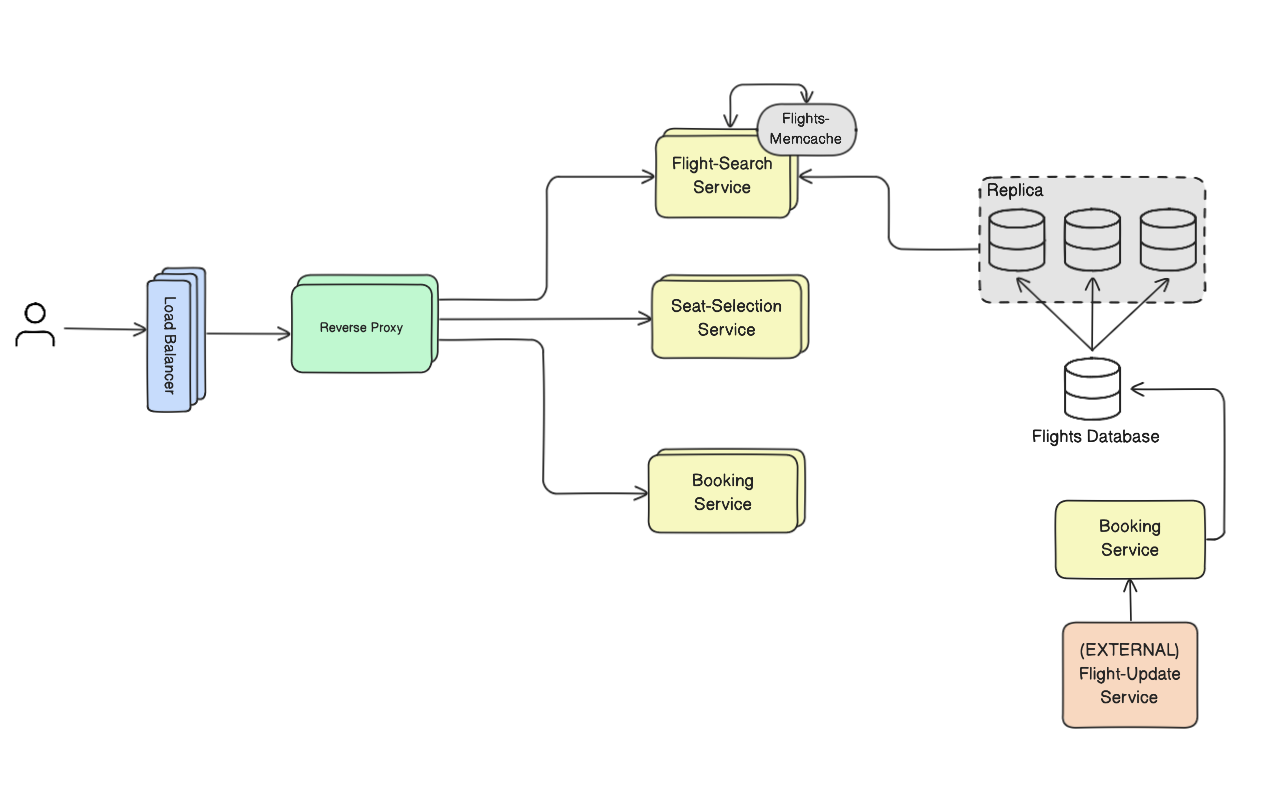
\includegraphics[width=\linewidth]{images/1st_system_design_sketch.png}
    \caption{Redesigned flight booking system (FBS)}
    \label{fig:fbs_design}
\end{figure}
\newpage 

\subsection{Discussion}
The functional requirements are mainly implemented as micro-services.
The Flight-Search service queries the database according to the users flight-data. The booking service is used to book a flight that 

The Seat-Select service is called if a customer wants to make a seat reservation on a selected plane. 
The proxy handles...security before forwarding to service, also record performance metrics as entry-point???

In order to address the non-functional requirements and insure scalability and performance different measures were taken. 
The Load-Balancer distributes the incoming traffic equally to the proxy-servers so that the performance of the system isn't impacted by a single overloaded server (that would take way to long to respond to the user-requests). This also enables another point of scalability such that we can increase the number of proxy servers if the overall workload is to high.
My analysis of the given flight-booking-system was, that it has a high write-to-read ratio (meaning the number of writes is way higher than the number of reads). Therefore we have database dublicates that all follow a single leader. With the additional caching it is insured, that the database-reads don't bottleneck the application. In the future additional replica can be added to support the database layer. We could also add additional partitioning (by origin-destination). 

To scale the micro-services it is always possible to horizontally scale the micro-services by adding more instances. If the request arrives at the service it will be load-balanced internally and send to one of its instances.


\section{Freestyle Exercise}
\subsection{My DS-Concept}
I chose to implement a distributed version of our assignment server. 
The core improvement is, that the workload is distributed amongst various stateless servers that can access a database to update a representative "assignment-01"-score. To scale the number of servers horizontally, I implemented a loadbalancer that uses round-robin scheduling to distributes the work amongst the registered servers. The idea is that the clients can only communicate with the servers via the loadbalancer, that forwards the workload, therefore increasing the maximum number of requests that can be processed in parallel. 
To represent a distributed system on a local machine, I wrote a docker-compose file. This file includes multiple servers in different networks (net-1 and net-2; representing two data-centers) as well as references to the loadbalancer, the database storing the student data and an API. The API is used to read certain database information and ultimately display the students and the passed/failed exam-entries in a neat static front-end[\ref{fig:frontend}].

\begin{figure}[!hb]
    \centering
    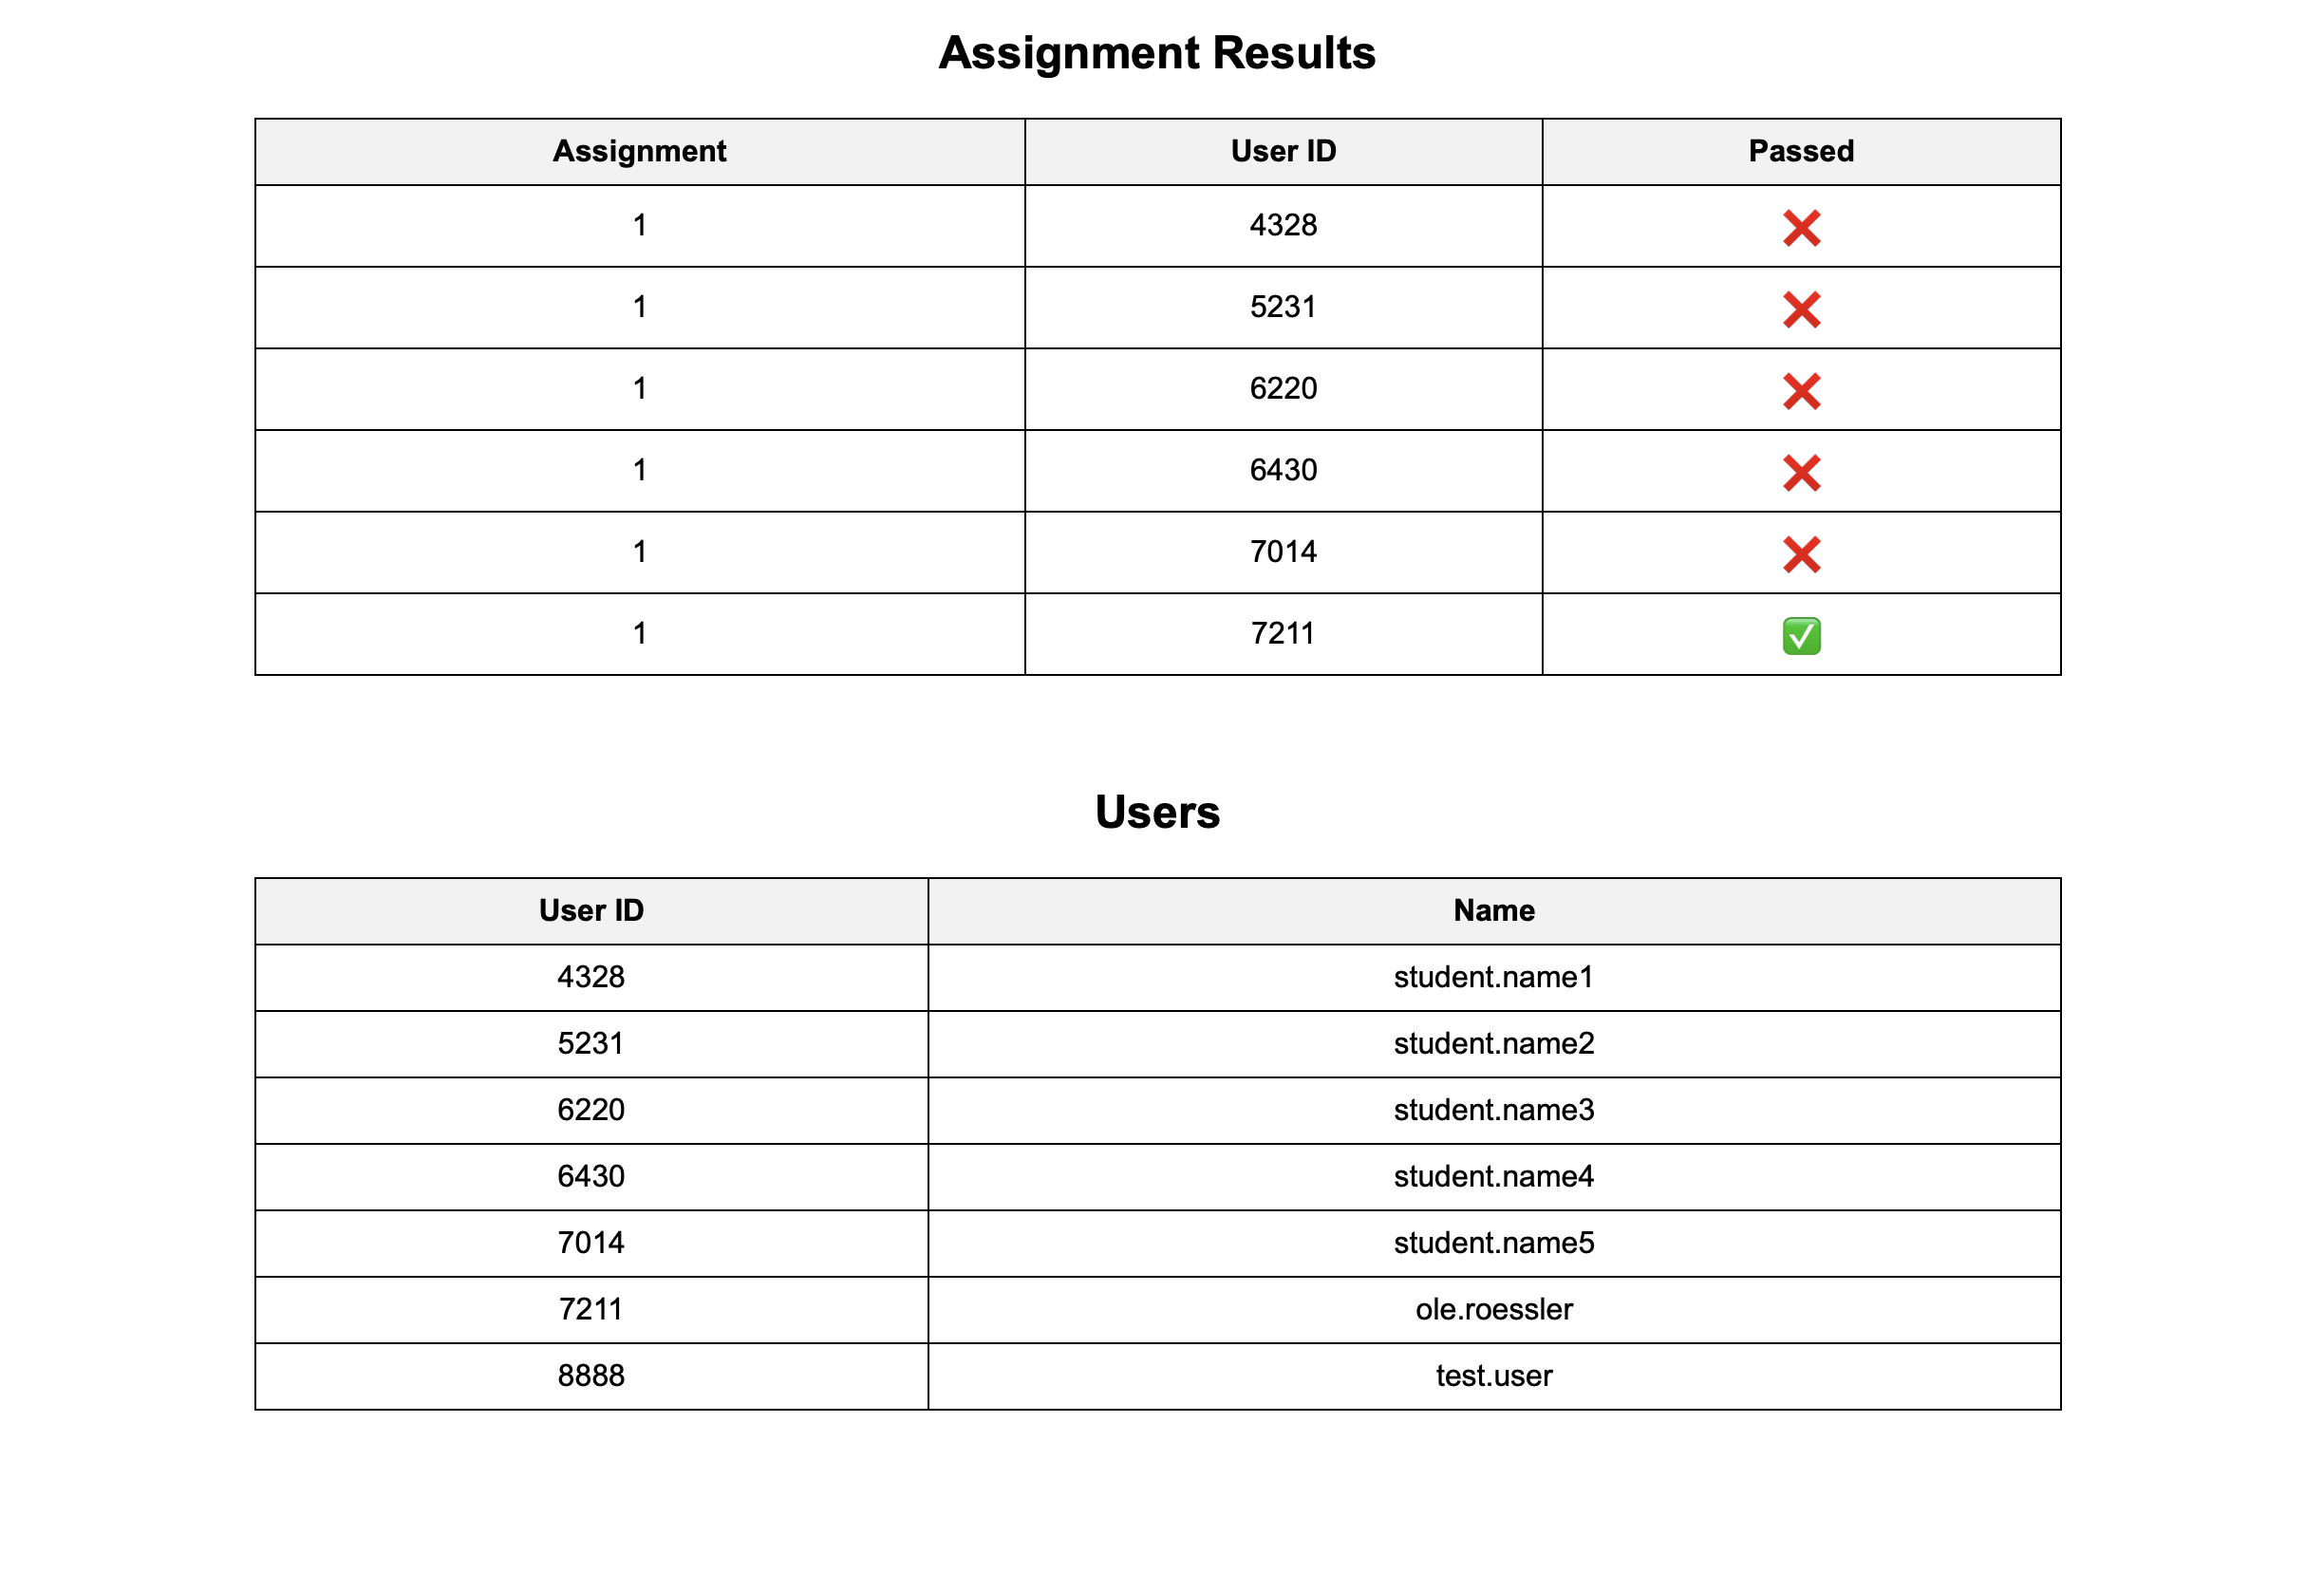
\includegraphics[width=1\linewidth]{images/frontend_screenshot.png}
    \caption{Screenshot of the front-end}
    \label{fig:frontend}
\end{figure}

I also implemented  a heart-beat mechanism that sends a udp-package from the servers to the loadbalancer every few seconds to signal that they are still alive and able to receive new data. 
I supported the processing of MessageTypes specified in the given ds-repo. 
The idea is, that the servers process given message-data and are able to write "assignment passed" or "assignment failed" into the database.
As it's only a prototype, I implemented a very easy test to simulate the behaviour of the real test-server:
If the received ChatMessage equals 'TEST 1 USER ID: ' + UID and the userId equals the userId specified in the ChatMessage the test gets passed. The server will return a message contaning "TEST 1 USER ID CORRECTNESS FAILED/PASSED", depending on the results of the message analysis. By the way, all other ChatMessages are just echoed.
Therefore the database only needs a table to save the assignment-scores as well as a table for all the registered users, as well as a few constraints(e.g. only one entry per user per assignment, only valid userIds in the assignments table).
The resulting postgresql database-schema looks accordingly[\ref{fig:database_assignment}].

\begin{figure}[!hb]
    \centering
    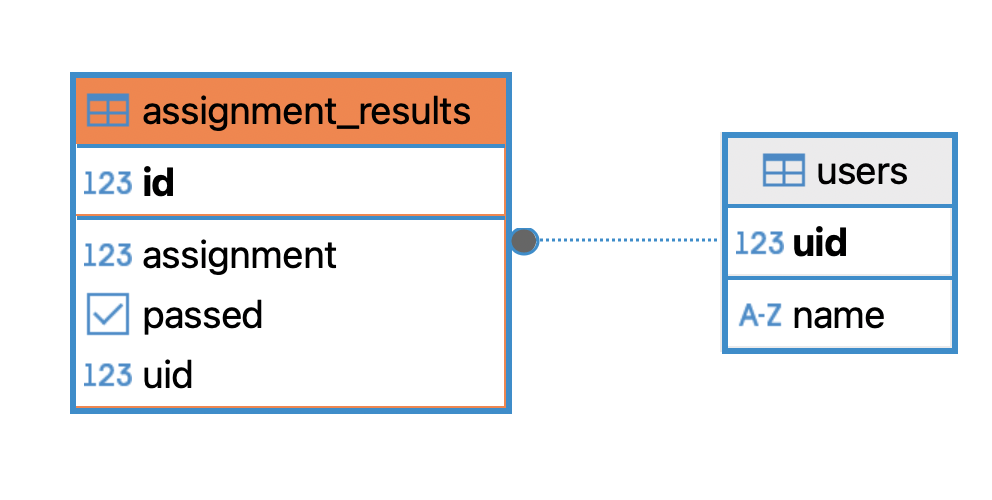
\includegraphics[width=0.5\linewidth]{images/database_screenshot.png}
    \caption{Enter Caption}
    \label{fig:database_assignment}
\end{figure}


To create a better overview of the created docker-compose "system", I included a screenshot of the running application in docker-desktop. We can see 3 different servers, a loadbalancer, the database as well as the api containers. The different servernodes are all running the same server-image but use different ports of receive data that was forwarded by the loadbalancer.
The database instance is just a postgres-14:alpina container specified to allow connections via the db-net. For further details consult the dockerfiles as well as the docker-compose file and the source-code.

\begin{figure}[!hb]
    \centering
    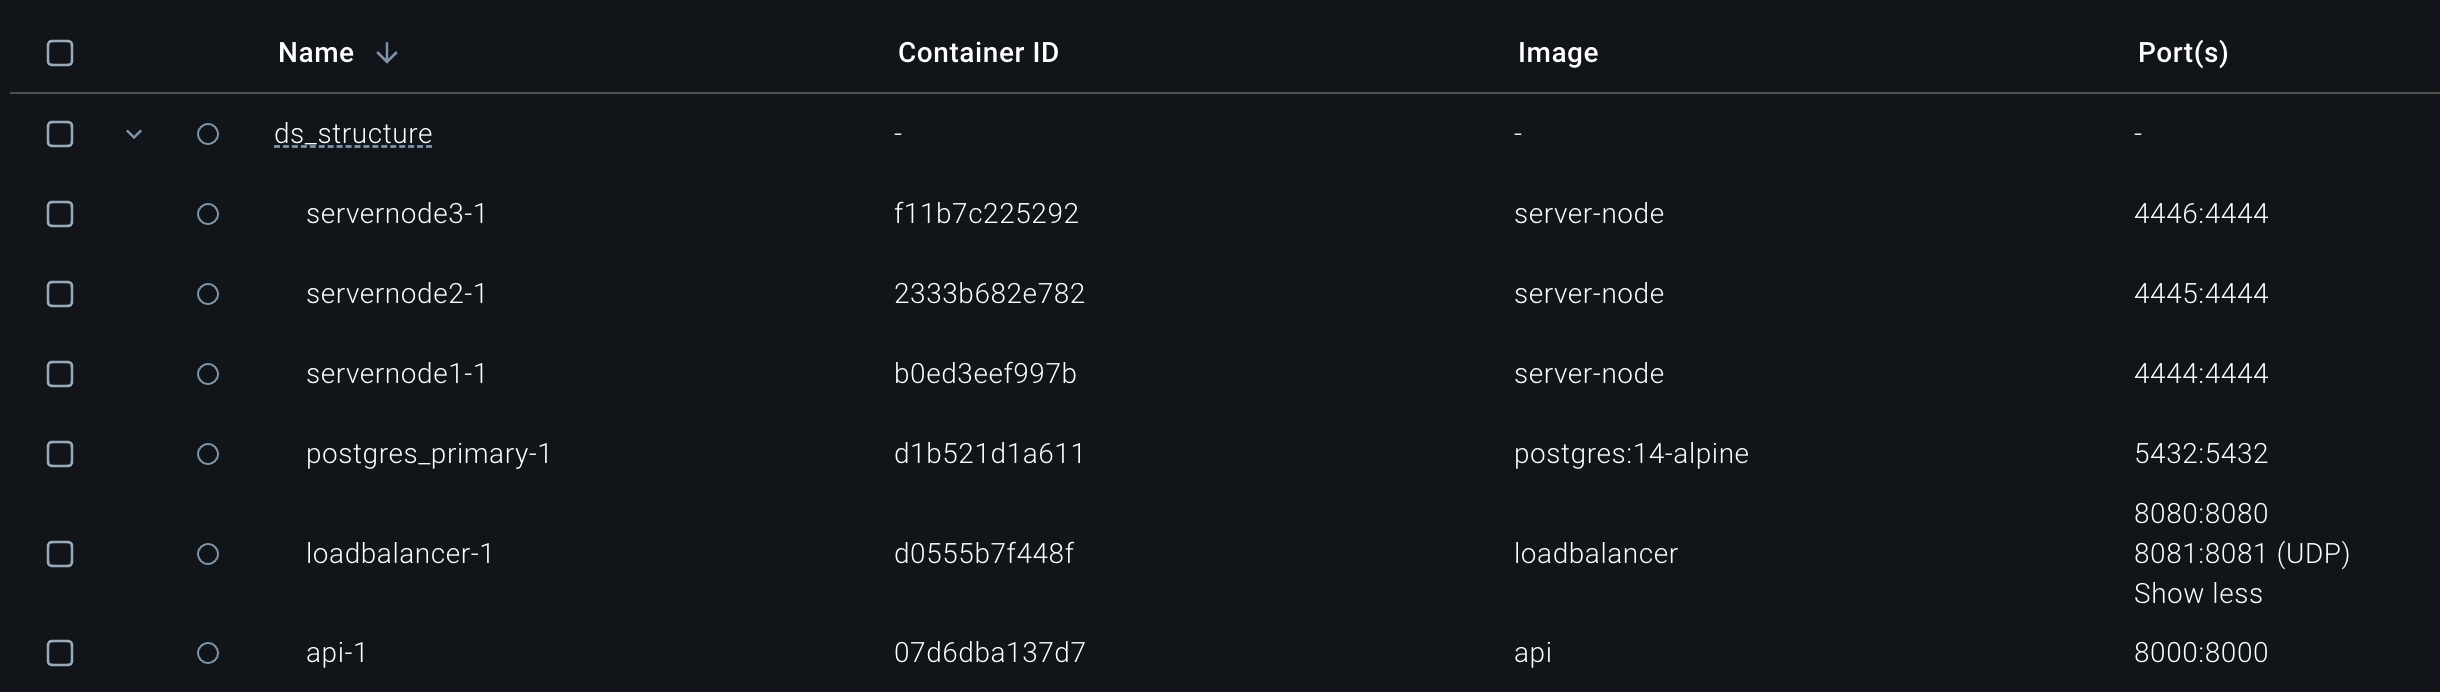
\includegraphics[width=1\linewidth]{images/docker_compose_screenshot.png}
    \caption{Screenshot of components via docker-desktop}
    \label{fig:docker_compose}
\end{figure}

\newpage

\subsection{Evaluation}
\subsubsection{Cons and Limitations}
\begin{enumerate}

\item \textbf{Suboptimal Load Balancing:}
Although round-robin is simple, it does not account for the actual server utilization. More advanced techniques like dynamic load balancing could distribute requests more efficiently when workloads are uneven across different requests. Especially when more complex test-cases are implemented, the workload might differ a lot (simple string comparison vs multi-step message protocol).

\item \textbf{Security Weaknesses:}
Even though this is only a prototype, it has to be mentioned that I didn't consider security at all.
The API currently lacks authentication (e.g., bearer tokens) and all ports are exposed through localhost. In a real environment the student should only have access to the loadbalancer and every following request, even to the server should include some sort of authentication.




\textbf{View Flights:}
The customer is able to see specific flight details. 
Therefore the customer enters a specific flight number/ flight ID and gets updates about the specified flight.
\item \textbf{Booking:}
The customer is able to book a flight on a desired flight as well as make a seat reservation on the airplane (Most airlines offer different price-tiers for seats). 
\end{enumerate}



Round-robin loadbalancing is enough for our usecase, but can could be more optimal(utilization based).

Pros:
read/write balance is good, way less writes than reads, therefore single leader is enough for handliung the writes.

Reads is way higher, because (problem, currently i write even on fail). 
HEARTBEAT:
- If a server is shut down or physically seperated from the load-balancer for any reason, the implemented udp-heartbeat can't be received by the load-balancer. Therefore the server is removed from the list of servers, participating in the round-robin.
servers



->Discussion Points
-idea: meh, why its enought, ids go up to 1000, so there are almost definitely less than 1000 users. So the one provided server would most definitely be enough to handle the peak traffic. But as I understand it, the idea was to have some fun with distributed systems and to build on the given communication protocol and \textit{"designing a novel application"}\cite{ds_4} 


-functional-requirements -> reasy to meat > not to complex: send data/save results/
-nonfunctional-req -> problem
big minus SECURITY:
-> API has no verificaction e.g. bearer token,e.g.
-> Single point of failure in loadbalancer and 

REQUIREMENTS
-> longr testcases need to be stored in db???? no longer connections between server and client
->ANALYSIS of requirements is probably wrong.

Improvements:
-> Distributed database 
-> Modularity/Encapsiation: Have api layer between db and java servers

\printbibliography[heading=bibintoc]
\end{document}